\chapter{Architecture Analysis}
\label{ch:architecture_analysis}

\section{Library Dependency Analysis}
\label{sec:library_dependency}

The \rus{} system exhibits a clear hierarchical dependency structure that enables modular development while maintaining system coherence. Figure \ref{fig:dependency_graph} illustrates the dependency relationships between core libraries.

\begin{figure}[H]
\centering
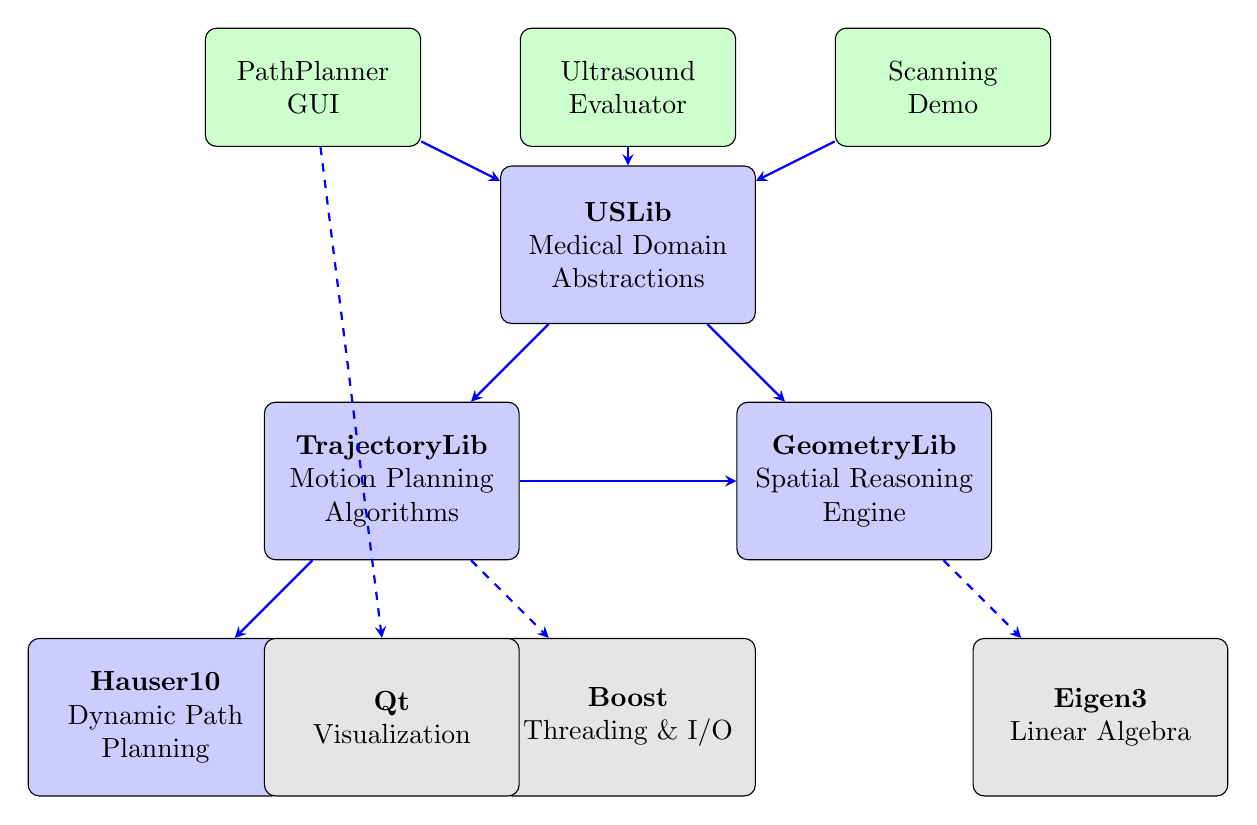
\begin{tikzpicture}[
    library/.style={rectangle, draw, fill=blue!20, text width=3cm, text centered, minimum height=2cm, rounded corners},
    dependency/.style={->, thick, blue, >=stealth},
    application/.style={rectangle, draw, fill=green!20, text width=2.5cm, text centered, minimum height=1.5cm, rounded corners}
]

% Libraries
\node[library] (uslib) at (0,6) {\textbf{USLib}\\Medical Domain\\Abstractions};
\node[library] (trajlib) at (-3,3) {\textbf{TrajectoryLib}\\Motion Planning\\Algorithms};
\node[library] (geolib) at (3,3) {\textbf{GeometryLib}\\Spatial Reasoning\\Engine};
\node[library] (hauser) at (-6,0) {\textbf{Hauser10}\\Dynamic Path\\Planning};

% Applications
\node[application] (pathplanner) at (-4,8) {PathPlanner\\GUI};
\node[application] (evaluator) at (0,8) {Ultrasound\\Evaluator};
\node[application] (demo) at (4,8) {Scanning\\Demo};

% Dependencies
\draw[dependency] (uslib) -- (trajlib);
\draw[dependency] (uslib) -- (geolib);
\draw[dependency] (trajlib) -- (geolib);
\draw[dependency] (trajlib) -- (hauser);

% Application dependencies
\draw[dependency] (pathplanner) -- (uslib);
\draw[dependency] (evaluator) -- (uslib);
\draw[dependency] (demo) -- (uslib);

% External dependencies
\node[library, fill=gray!20] (eigen) at (6,0) {\textbf{Eigen3}\\Linear Algebra};
\node[library, fill=gray!20] (boost) at (0,0) {\textbf{Boost}\\Threading \& I/O};
\node[library, fill=gray!20] (qt) at (-3,0) {\textbf{Qt}\\Visualization};

\draw[dependency, dashed] (geolib) -- (eigen);
\draw[dependency, dashed] (trajlib) -- (boost);
\draw[dependency, dashed] (pathplanner) -- (qt);

\end{tikzpicture}
\caption{Library Dependency Graph}
\label{fig:dependency_graph}
\end{figure}

\subsection{Dependency Characteristics}

\begin{description}
    \item[USLib $\rightarrow$ TrajectoryLib] Medical domain logic depends on generic motion planning capabilities for trajectory generation and optimization.
    
    \item[USLib $\rightarrow$ GeometryLib] Ultrasound-specific algorithms require spatial reasoning for collision detection and workspace analysis.
    
    \item[TrajectoryLib $\rightarrow$ GeometryLib] Motion planning algorithms utilize geometric computations for obstacle avoidance and path validation.
    
    \item[TrajectoryLib $\rightarrow$ Hauser10] Integration with dynamic path planning library for time-optimal trajectory generation.
\end{description}

\section{Component Interaction Patterns}
\label{sec:interaction_patterns}

The \rus{} architecture implements several sophisticated interaction patterns that facilitate loose coupling while maintaining high performance.

\subsection{Observer Pattern Implementation}

Real-time monitoring and event propagation utilize the Observer pattern for asynchronous communication:

\begin{lstlisting}[caption={Observer Pattern for Trajectory Monitoring}, label={lst:observer_pattern}]
class TrajectoryExecutionObserver {
public:
    virtual void onTrajectoryStarted(const TrajectoryInfo& info) = 0;
    virtual void onTrajectoryProgress(double progress, 
                                     const RobotState& state) = 0;
    virtual void onTrajectoryCompleted(const TrajectoryResult& result) = 0;
    virtual void onTrajectoryError(const ErrorInfo& error) = 0;
    virtual void onForceThresholdExceeded(const ForceReading& force) = 0;
    virtual ~TrajectoryExecutionObserver() = default;
};

class TrajectoryExecutor {
private:
    std::vector<std::shared_ptr<TrajectoryExecutionObserver>> _observers;
    
public:
    void addObserver(std::shared_ptr<TrajectoryExecutionObserver> observer) {
        _observers.push_back(observer);
    }
    
    void notifyTrajectoryProgress(double progress, const RobotState& state) {
        for (auto& observer : _observers) {
            observer->onTrajectoryProgress(progress, state);
        }
    }
};
\end{lstlisting}

\subsection{Strategy Pattern for Algorithm Selection}

The system employs the Strategy pattern for runtime algorithm selection:

\begin{lstlisting}[caption={Strategy Pattern for Motion Planning}, label={lst:strategy_pattern}]
class MotionPlanningStrategy {
public:
    virtual TrajectoryResult plan(const RobotArm& arm,
                                 const std::vector<Eigen::Affine3d>& poses,
                                 const Environment& env) = 0;
    virtual std::string getName() const = 0;
    virtual ParameterMap getParameters() const = 0;
    virtual void setParameters(const ParameterMap& params) = 0;
    virtual ~MotionPlanningStrategy() = default;
};

class STOMPStrategy : public MotionPlanningStrategy {
private:
    StompConfig _config;
    std::unique_ptr<MotionGenerator> _generator;
    
public:
    TrajectoryResult plan(const RobotArm& arm,
                         const std::vector<Eigen::Affine3d>& poses,
                         const Environment& env) override {
        _generator->setWaypoints(convertPosesToWaypoints(poses));
        bool success = _generator->performSTOMP(_config);
        return TrajectoryResult{_generator->getPath(), success};
    }
};
\end{lstlisting}

\subsection{Command Pattern for Undo/Redo Operations}

Trajectory planning operations implement the Command pattern for operation reversibility:

\begin{lstlisting}[caption={Command Pattern for Trajectory Operations}, label={lst:command_pattern}]
class TrajectoryCommand {
public:
    virtual bool execute() = 0;
    virtual bool undo() = 0;
    virtual bool redo() = 0;
    virtual std::string getDescription() const = 0;
    virtual ~TrajectoryCommand() = default;
};

class PlanTrajectoryCommand : public TrajectoryCommand {
private:
    UltrasoundScanTrajectoryPlanner* _planner;
    std::vector<Eigen::Affine3d> _poses;
    std::vector<TrajectoryPoint> _previousTrajectory;
    std::vector<TrajectoryPoint> _newTrajectory;
    
public:
    bool execute() override {
        _previousTrajectory = _planner->getTrajectories();
        _planner->setPoses(_poses);
        bool success = _planner->planTrajectories();
        if (success) {
            _newTrajectory = _planner->getTrajectories();
        }
        return success;
    }
    
    bool undo() override {
        _planner->setTrajectories(_previousTrajectory);
        return true;
    }
};
\end{lstlisting}

\section{Data Flow Architecture}
\label{sec:data_flow}

\subsection{Multi-Stream Data Processing}

The \rus{} system processes multiple concurrent data streams with varying priorities and timing requirements:

\begin{figure}[H]
\centering
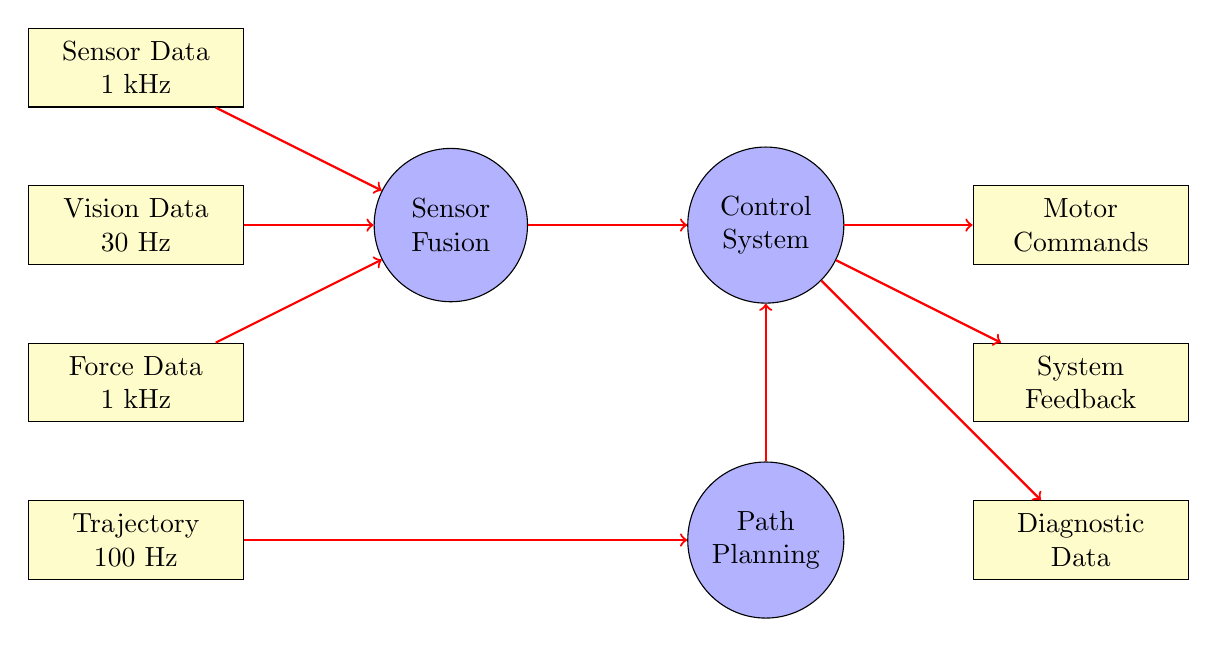
\begin{tikzpicture}[
    stream/.style={rectangle, draw, fill=yellow!20, text width=2.5cm, text centered, minimum height=1cm},
    processor/.style={circle, draw, fill=blue!30, text width=1.5cm, text centered},
    flow/.style={->, thick, red}
]

% Data streams
\node[stream] (sensor) at (-6,4) {Sensor Data\\1 kHz};
\node[stream] (vision) at (-6,2) {Vision Data\\30 Hz};
\node[stream] (force) at (-6,0) {Force Data\\1 kHz};
\node[stream] (trajectory) at (-6,-2) {Trajectory\\100 Hz};

% Processors
\node[processor] (fusion) at (-2,2) {Sensor\\Fusion};
\node[processor] (control) at (2,2) {Control\\System};
\node[processor] (planning) at (2,-2) {Path\\Planning};

% Outputs
\node[stream] (commands) at (6,2) {Motor\\Commands};
\node[stream] (feedback) at (6,0) {System\\Feedback};
\node[stream] (diagnostics) at (6,-2) {Diagnostic\\Data};

% Data flows
\draw[flow] (sensor) -- (fusion);
\draw[flow] (vision) -- (fusion);
\draw[flow] (force) -- (fusion);
\draw[flow] (trajectory) -- (planning);

\draw[flow] (fusion) -- (control);
\draw[flow] (planning) -- (control);

\draw[flow] (control) -- (commands);
\draw[flow] (control) -- (feedback);
\draw[flow] (control) -- (diagnostics);

\end{tikzpicture}
\caption{Multi-Stream Data Flow Architecture}
\label{fig:data_flow}
\end{figure}

\subsection{Temporal Synchronization}

Data streams with different sampling rates require careful temporal synchronization:

\begin{equation}
t_{sync} = \max(t_1, t_2, \ldots, t_n) + \Delta t_{latency}
\end{equation}

where $t_i$ represents the timestamp of data stream $i$ and $\Delta t_{latency}$ accounts for processing delays.

\section{Memory Architecture}
\label{sec:memory_architecture}

\subsection{Memory Hierarchy Optimization}

The \rus{} system implements a sophisticated memory hierarchy to optimize performance:

\begin{table}[H]
\centering
\caption{Memory Hierarchy Characteristics}
\label{tab:memory_hierarchy}
\begin{tabular}{@{}lcccc@{}}
\toprule
\textbf{Memory Level} & \textbf{Size} & \textbf{Latency} & \textbf{Bandwidth} & \textbf{Usage} \\
\midrule
L1 Cache & 32 KB & 1 cycle & 1000 GB/s & Hot data \\
L2 Cache & 256 KB & 3-4 cycles & 500 GB/s & Frequently accessed \\
L3 Cache & 8 MB & 10-20 cycles & 100 GB/s & Shared data \\
Main Memory & 32 GB & 100-300 cycles & 50 GB/s & Primary storage \\
SSD Storage & 1 TB & 100,000 cycles & 3 GB/s & Persistent data \\
\bottomrule
\end{tabular}
\end{table}

\subsection{Cache-Optimized Data Structures}

The system employs Structure-of-Arrays (SoA) patterns for improved cache locality:

\begin{lstlisting}[caption={Cache-Optimized Trajectory Storage}, label={lst:cache_optimization}]
class TrajectoryPointArray {
private:
    // Separate arrays for better cache performance
    std::vector<double> _timestamps;        // Temporal data
    std::vector<double> _positions;         // Joint positions (7 * N)
    std::vector<double> _velocities;        // Joint velocities (7 * N)
    std::vector<double> _accelerations;     // Joint accelerations (7 * N)
    
    size_t _numPoints;
    size_t _numJoints = 7;
    
public:
    // Cache-friendly accessors
    double getPosition(size_t pointIndex, size_t jointIndex) const {
        return _positions[pointIndex * _numJoints + jointIndex];
    }
    
    // Vectorized operations for SIMD optimization
    void computeVelocities(double dt) {
        const size_t totalSize = _numPoints * _numJoints;
        
        #pragma omp simd
        for (size_t i = _numJoints; i < totalSize; ++i) {
            _velocities[i] = (_positions[i] - _positions[i - _numJoints]) / dt;
        }
    }
};
\end{lstlisting}

\section{Concurrency Architecture}
\label{sec:concurrency_architecture}

\subsection{Thread Pool Management}

The system implements sophisticated thread pool management for optimal resource utilization:

\begin{lstlisting}[caption={Advanced Thread Pool Management}, label={lst:thread_pool}]
class ThreadPoolManager {
private:
    std::shared_ptr<boost::asio::thread_pool> _stompPool;
    std::shared_ptr<boost::asio::thread_pool> _collisionPool;
    std::shared_ptr<boost::asio::thread_pool> _visualizationPool;
    
    struct ThreadPoolConfig {
        size_t stompThreads = 2 * std::thread::hardware_concurrency();
        size_t collisionThreads = std::thread::hardware_concurrency();
        size_t visualizationThreads = 4;
        
        ThreadPriority stompPriority = ThreadPriority::HIGH;
        ThreadPriority collisionPriority = ThreadPriority::REALTIME;
        ThreadPriority visualizationPriority = ThreadPriority::NORMAL;
    } _config;
    
public:
    void initializeThreadPools() {
        _stompPool = std::make_shared<boost::asio::thread_pool>(_config.stompThreads);
        _collisionPool = std::make_shared<boost::asio::thread_pool>(_config.collisionThreads);
        _visualizationPool = std::make_shared<boost::asio::thread_pool>(_config.visualizationThreads);
        
        // Set thread priorities (platform-specific implementation)
        setThreadPoolPriority(_stompPool, _config.stompPriority);
        setThreadPoolPriority(_collisionPool, _config.collisionPriority);
        setThreadPoolPriority(_visualizationPool, _config.visualizationPriority);
    }
    
    template<typename Function>
    auto submitSTOMPTask(Function&& f) -> std::future<decltype(f())> {
        auto task = std::make_shared<std::packaged_task<decltype(f())()>>(
            std::forward<Function>(f)
        );
        
        auto future = task->get_future();
        boost::asio::post(*_stompPool, [task]() { (*task)(); });
        
        return future;
    }
};
\end{lstlisting}

\subsection{Lock-Free Data Structures}

For high-performance inter-thread communication, the system employs lock-free data structures:

\begin{lstlisting}[caption={Lock-Free Ring Buffer Implementation}, label={lst:lockfree_buffer}]
template<typename T, size_t CAPACITY>
class LockFreeRingBuffer {
private:
    std::array<T, CAPACITY> _buffer;
    std::atomic<size_t> _writeIndex{0};
    std::atomic<size_t> _readIndex{0};
    
    static constexpr size_t MASK = CAPACITY - 1;
    static_assert((CAPACITY & MASK) == 0, "Capacity must be power of 2");
    
public:
    bool tryPush(const T& item) {
        const size_t currentWrite = _writeIndex.load(std::memory_order_relaxed);
        const size_t nextWrite = (currentWrite + 1) & MASK;
        
        if (nextWrite == _readIndex.load(std::memory_order_acquire)) {
            return false;  // Buffer full
        }
        
        _buffer[currentWrite] = item;
        _writeIndex.store(nextWrite, std::memory_order_release);
        return true;
    }
    
    bool tryPop(T& item) {
        const size_t currentRead = _readIndex.load(std::memory_order_relaxed);
        
        if (currentRead == _writeIndex.load(std::memory_order_acquire)) {
            return false;  // Buffer empty
        }
        
        item = _buffer[currentRead];
        _readIndex.store((currentRead + 1) & MASK, std::memory_order_release);
        return true;
    }
    
    size_t approximateSize() const {
        const size_t write = _writeIndex.load(std::memory_order_acquire);
        const size_t read = _readIndex.load(std::memory_order_acquire);
        return (write - read) & MASK;
    }
};
\end{lstlisting}

\section{Error Propagation and Handling}
\label{sec:error_propagation}

\subsection{Exception Hierarchy}

The system implements a comprehensive exception hierarchy for structured error handling:

\begin{lstlisting}[caption={Comprehensive Exception Hierarchy}, label={lst:exception_hierarchy}]
namespace RobotSystem {
    class RobotSystemException : public std::exception {
    private:
        std::string _message;
        ErrorCode _errorCode;
        std::string _context;
        std::chrono::system_clock::time_point _timestamp;
        std::vector<std::string> _stackTrace;
        
    public:
        RobotSystemException(ErrorCode code, 
                           const std::string& message,
                           const std::string& context = "")
            : _errorCode(code)
            , _message(message)
            , _context(context)
            , _timestamp(std::chrono::system_clock::now()) {
            captureStackTrace();
        }
        
        const char* what() const noexcept override { 
            return _message.c_str(); 
        }
        
        ErrorCode getErrorCode() const { return _errorCode; }
        const std::string& getContext() const { return _context; }
        auto getTimestamp() const { return _timestamp; }
        const std::vector<std::string>& getStackTrace() const { 
            return _stackTrace; 
        }
        
    private:
        void captureStackTrace();
    };
    
    // Specialized exception types
    class TrajectoryPlanningException : public RobotSystemException {
    private:
        StompConfig _config;
        std::vector<Eigen::Affine3d> _poses;
        
    public:
        TrajectoryPlanningException(const std::string& message,
                                  const StompConfig& config,
                                  const std::vector<Eigen::Affine3d>& poses)
            : RobotSystemException(ErrorCode::TRAJECTORY_PLANNING_FAILED, message)
            , _config(config)
            , _poses(poses) {}
            
        const StompConfig& getConfig() const { return _config; }
        const std::vector<Eigen::Affine3d>& getPoses() const { return _poses; }
    };
    
    class CollisionException : public RobotSystemException {
    private:
        Eigen::Vector3d _collisionPoint;
        double _penetrationDepth;
        std::string _objectName;
        
    public:
        CollisionException(const Eigen::Vector3d& point, 
                         double depth,
                         const std::string& objectName = "")
            : RobotSystemException(ErrorCode::COLLISION_DETECTED,
                                 "Collision detected during trajectory execution")
            , _collisionPoint(point)
            , _penetrationDepth(depth)
            , _objectName(objectName) {}
            
        const Eigen::Vector3d& getCollisionPoint() const { 
            return _collisionPoint; 
        }
        double getPenetrationDepth() const { return _penetrationDepth; }
        const std::string& getObjectName() const { return _objectName; }
    };
}
\end{lstlisting}

\subsection{Graceful Degradation Strategy}

The system implements adaptive performance management for graceful degradation:

\begin{lstlisting}[caption={Adaptive Performance Management}, label={lst:performance_management}]
class AdaptivePerformanceManager {
private:
    struct PerformanceMetrics {
        double averagePlanningTime = 0.0;
        double memoryUsage = 0.0;
        double cpuUtilization = 0.0;
        size_t failureCount = 0;
        std::chrono::steady_clock::time_point lastUpdate;
    } _metrics;
    
    StompConfig _baseConfig;
    StompConfig _currentConfig;
    
public:
    enum class PerformanceMode {
        OPTIMAL,        // Full performance, all features enabled
        BALANCED,       // Good performance, some features reduced
        CONSERVATIVE,   // Reduced performance, enhanced stability
        MINIMAL         // Basic functionality only
    };
    
    void updatePerformanceMode() {
        PerformanceMode newMode = determineOptimalMode();
        
        switch (newMode) {
            case PerformanceMode::OPTIMAL:
                _currentConfig = _baseConfig;
                break;
                
            case PerformanceMode::BALANCED:
                _currentConfig.numNoisyTrajectories = 
                    std::max(2, _baseConfig.numNoisyTrajectories / 2);
                _currentConfig.maxIterations = 
                    static_cast<int>(_baseConfig.maxIterations * 0.8);
                break;
                
            case PerformanceMode::CONSERVATIVE:
                _currentConfig.numNoisyTrajectories = 
                    std::max(2, _baseConfig.numNoisyTrajectories / 4);
                _currentConfig.maxIterations = 
                    static_cast<int>(_baseConfig.maxIterations * 0.6);
                _currentConfig.dt *= 1.5;  // Coarser discretization
                break;
                
            case PerformanceMode::MINIMAL:
                _currentConfig.numNoisyTrajectories = 2;
                _currentConfig.maxIterations = 50;
                _currentConfig.dt *= 2.0;
                break;
        }
        
        logPerformanceModeChange(newMode);
    }
    
private:
    PerformanceMode determineOptimalMode() const {
        if (_metrics.averagePlanningTime > 10.0 || _metrics.memoryUsage > 0.8) {
            return PerformanceMode::CONSERVATIVE;
        }
        if (_metrics.failureCount > 3) {
            return PerformanceMode::MINIMAL;
        }
        if (_metrics.cpuUtilization > 0.9) {
            return PerformanceMode::BALANCED;
        }
        return PerformanceMode::OPTIMAL;
    }
};
\end{lstlisting}
